\documentclass{article}

\usepackage[utf8]{inputenc}
\usepackage[ngerman]{babel}
\usepackage{amsmath}
\usepackage{url}
\usepackage[pdftex]{graphicx}
\usepackage{listings}
 
\title{Object Caching\\Project Proposal}
\author{Lukas Hofmaier, Raphael Kohler, Timon Brüllmann}
\date{\today}
\begin{document}
\maketitle
\section{Betreuer}
J.M.Joller  Abteilung für Informatik HSR/FHO

\section{Motivation}
Das Datenverarbeitungssystem Mercury ermöglicht es Methoden von Objekten über mehrere Clients aufzurufen. Dabei treten unter anderem folgende Probleme auf:

\begin{itemize}
\item Clients können Werte von Instanzvariablen von Objekten auf dem Server lesen. Nutzt der Client diese Werte als Argumente in kausal Abhängigen Methoden kann ein Lost Update auftreten.
\item Alle Methodenaufrufe werden über das Netzwerk an den Server gesendet. Die Methodenaufrufe auf den Clients sollen schneller werden.
\end{itemize}

\section{Ziele der Arbeit}

\subsection{Hauptziele}
\label{sec:hauptziele}

\subsubsection{RMI mit Concurrency Control}
\label{sec:rmi-mit-concurrency}

In dieser Semesterarbeit soll nun ein Konzept erarbeitet werden, welches Lost Updates bei kausal abhängigen Methoden verhindert.  Es soll ein vereinfachtes RMI System implementiert werden. Dieses System soll zeigen, ob sich das Konzept einfach realisieren lässt.

\subsubsection{Testframework}
\label{sec:testframework}

Um das System zu testen, wird parallel dazu ein Testframework entwickelt. Das dieses Framework soll in der Lage sein unterschiedliche RMI System als Server und Client zu starten. Das Testframework ist in der Lage eine Szenariobeschreibung einzulesen und dieses Szenario mit dem zu testenden System durchzuspielen. Es sammelt dabei Messdaten über die Zeitdauer der einzelnen Methodenaufrufe. Die Messdaten sollen es ermöglichen, abzuwägen welche Systeme mit welchen Parameter sich für welchen Anwendungszweck eignen.
Das Testframework registriert das Auftreten von Schreib-Konfikten bei Aufruf von Schreibmethoden.

\subsection{Erweiterte Ziele}
\label{sec:erweiterte-ziele}

\subsubsection{Object Caching}
\label{sec:object-caching}

Um die Dauer von Methodenaufrufen zu verkürzen, soll das RMI System um einen Object Cache erweitert werden. Methoden ohne Seiteneffekte werden auf den Objekten im Cache ausgeführt. Für das System wird ein passendes Konsistenzmodell ausgewählt. Dieses Modell wird durch ein geeignetes Konsistenzprotokoll durchgesetzt. Die Unterscheidung von Lese und Schreib- Methoden muss durch den User gemacht werden.

\subsubsection{Feingranulares Locking}
\label{sec:feingr-lock}

Das System RMI mit Concurrency Control setzt Thread-Synchronisierung ein. Das System soll so konzipiert und implementiert werden, dass möglichst viele Methoden innerhalb einer definierten Zeit ausgeführt werden können.

\subsection{Szenarien}
\label{sec:szenario}

Als Ausgangslage für das gesamte Projekt wird folgendes Szenario eingesetzt:

Es wird ein verteiltes System mit einem Server und zwei Clients verwendet.
\begin{center}
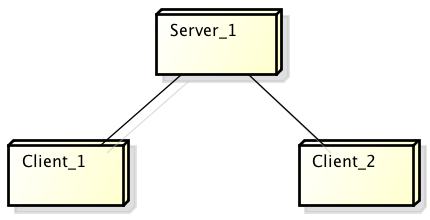
\includegraphics[scale=0.85]{Deployment.png}
\end{center}

Die Clients möchten den Kontostand um 10 \% erhöhen. Sie führen dazu folgende Schritte aus
\begin{lstlisting}
b = getBalance();
setBalance( b * 1.1 );
\end{lstlisting}
Diese Schritte werden zum Prozess \"Kontostand Erhöhen\" zusammengefasst.

Auf einem Server wird ein Account-Objekt instanziert.
Das Interface von Account sieht wie folgt aus:
\begin{lstlisting}
public interface Account {
    public int getBalance();
    public void setBalance(int balance);    
}
\end{lstlisting}
Zwischen getBalance und setBalance besteht ein kausaler Zusammenhang. setBalance darf nur ausgeführt werden, wenn das Argument balance aktuell ist. Ist der Wert nicht mehr aktuell, wird der "Kontostand-Erhöhen"-Prozess abgebrochen. Der Client wiederholt in diesem Fall den gesamten Prozess (aktuelle Daten holen, Daten schreiben) noch automatisch.

Dem Client ist das Interface Account bekannt. Das Interface wird vor Prozessstart deployed.

Zwei Client beschaffen sich eine Referenz in Form eines Proxy-Objektes auf das Account-Objekt. 

Bei jedem Szenario werden folgende Messdaten festgehalten.
\begin{itemize}
\item durchschnittliche Dauer des Methodenaufrufs getBalance()
\item durchschnittliche Dauer des Methodenaufrufs setBalance()
\item Anzahl aufgetretene Konflikte
\item Dauer eines setBalance(); Methodenaufrufs bei Konfliktsituation
  \begin{itemize}
  \item Zeitdifferenz zwischen erstem setBalance bis erfolgreichem setBalance
  \item Zeitdifferenz zwischen setBalance und Empfang der zugehörigen Exception
  \end{itemize}
\end{itemize}

\subsubsection{Konfliktloser Zugriff}
\label{sec:konfl-zugr}

Das Szenario soll zeigen wie lange Methodenaufrufe dauern, wenn keine Konflikte auftreten. Ein Client führt den Prozess Kontostand-Erhöhen 10000-mal aus.

\subsubsection{Race Condition}
\label{sec:race-condition}
Das Szenario soll zeigen wie viele Konflikte auftreten, wenn beide Clients permanent Kontoerhöhungen ausführen wollen.
Beide Clients führen den Prozess Kontostand-Erhöhen 10000 mal aus. Server startet die Clients hintereinander mit einer möglichst kleinen Zeitdifferenz.

\subsubsection{Erzwungene Konflikte}
\label{sec:erzwungene-konflikte}

In diesem Szenario soll jeder setBalance-Aufruf von Client 2 zu einer Konfliktsituation führen. Damit sind Konfliktsituation nicht dem Zufall überlassen, sondern treten zuverlässig auf und können besser analysiert werden.

Client 1 führt ununterbrochen Kontoerhöhungen aus. Client 2 führt 100 Kontoerhöhungen aus. Client 2 wartet nach dem getBalance()-Aufruf 10ms. In dieser Zeit sollte Client1 eine Schreiboperation ausführen und die Daten im Speicher von Client 2 werden veraltet.

Im zweiten Teil der Semesterarbeit werden dann mehrere Account Objekte angelegt.



\section{Technologische Rahmenbedingungen}
Die Lösung wird in Java entwickelt und als externe Datendarstellung wird XML verwendet, diese bietet den grossen Vorteil von einer plattformneutralen Datendarstellung. Jegliche Sicherheitsaspekte sind nicht Thema dieser Semesterarbeit und sollen fürs erste nicht berücksichtigt werden (Zugriffskontrolle).

\section{Zur Ausführung}
Die erfolgreiche Bearbeitung dieser Aufgabe setzt Grundkenntnisse in der Programmierung verteilter Systeme voraus (praktische Beispiele, nicht bloss Literaturkenntnisse) sowie die Bereitschaft sich in neue und neuste Ergebnisse einzuarbeiten.
Mit dem Betreuer finden in der Regel wöchentliche Besprechungen statt. Zusätzliche Besprechungen sind nach Bedarf durch die Studierenden zu veranlassen. Das Sitzungsintervall ist flexibel: falls wenig oder keine Probleme auftreten können die Sitzungsintervalle vergrössert werden; falls Probleme auftauchen, werden die Intervalle verkleinert.\\
Alle Besprechungen sind von den Studenten mit einer Traktandenliste vorzubereiten und die Ergebnisse sind in einem Protokoll zu dokumentieren, das dem Betreuer per E-Mail zugestellt wird.\\
Für die Durchführung der Arbeit ist ein Projektplan zu erstellen. Dabei ist auf einen kontinuierlichen und sichtbaren Arbeitsfortschritt zu achten. An Meilensteinen gemäss Projektplan sind einzelne Arbeitsresultate in vorläufigen Versionen abzugeben. 
\section{Dokumentation und Abgabe}
Wegen der beabsichtigten Verwendung der Ergebnisse in weiteren Projekten wird auf Vollständigkeit sowie (sprachliche und grafische) Qualität der Dokumentation erhöhter Wert gelegt.\\
Die Dokumentation zur Projekt- Planung und –Verfolgung ist gemäss den Richtlinien der Abteilung Informatik anzufertigen. Die Detailanforderungen an die Dokumentation der Recherche- und Ent-wicklungsergebnisse werden entsprechend dem konkreten Arbeitsplan festgelegt.\\
Die Dokumentation ist vollständig auf CD abzugeben oder Zugriff auf eine Ablage (SVN, GIT).
Neben der Dokumentation sind abzugeben:
\begin{itemize}
\item alle zum Nachvollziehen der Arbeit notwendigen Ergebnisse und Daten (Quellcode, Buildskripte, Testcode, Testdaten usw.)
\item Material für eine Abschlusspräsentation (ca. 20’)
\end{itemize}

\section{Termine}

\begin{tabular}{l|ll}
Woche & Tasks \\ \hline
1 & Beginn der Studienarbeit; Kick-off Meeting bei Staila im Technopark \\
4 & Abgabe Project Proposal\\
5 & Phase 1 beendet; Test Framework sowie die „RMI with Coherence Control“ Lösung fertig.\\
12 &  Phase 2 beendet. „RMI with Cache“ fertig und getestet. \\
13 & Auswertung der Test Resultate
\end{tabular}

\section{Literaturhinweise}
Generelle Referenzen:\\
Siehe Vorlesung über Verteilte Software Systeme.\\
Weitere Literatur wird bei Bedarf zur Verfügung gestellt!
\section{Beurteilung}
Eine erfolgreiche Studienarbeit erhält 8 ECTS-Punkten (1 ECTS Punkt entspricht einer Arbeitsleistung von ca. 25 bis 30 Stunden). Für die Modulbeschreibung der Studienarbeit siehe 
\url{https://unterricht.hsr.ch/staticWeb/allModules/10938_M_SAI.html}.\\ \\
\begin{tabular}{l p{3cm} l l l}
Gesichtspunkt & Gewicht \\ \hline
1. Organisation, Durchführung & 1/5 \\
2. Berichte (Abstract, Management Summary, techn. u. persönliche Berichte) sowie Gliederung, Darstellung, Sprache der gesamten Dokumentation & 1/5 \\
3. Inhalt*) & 3/5
\end{tabular}
*) Die Unterteilung und Gewichtung von 3. Inhalt wird im Laufe dieser Arbeit mit dem Studenten vereinbart. Im Übrigen gelten die Bestimmungen der Abt. Informatik zur Durchführung von Studienarbeiten.\\ \\
Rapperswil, den\\
Der verantwortliche Dozent\\
\end{document}